% Modelo IEEE de conferência. Compila no Overleaf com pdfLaTeX e BibTeX.
% Arquivo único: todo o texto, as tabelas, o fluxograma e as referências estão aqui.
% As imagens ficam na pasta figuras/.
\documentclass[conference]{IEEEtran}
\usepackage[utf8]{inputenc}
\usepackage[T1]{fontenc}
\usepackage[brazil]{babel}
\usepackage{amsmath,amssymb}
\usepackage{graphicx}
\usepackage{booktabs}
\usepackage{multirow}
\usepackage{subcaption}
\usepackage{algorithm}
\usepackage{algpseudocode}
\usepackage{tikz}
\usetikzlibrary{positioning,arrows.meta}
\usepackage{url}
\usepackage{xcolor}

\floatname{algorithm}{Algoritmo}
\renewcommand{\algorithmicrequire}{\textbf{Entrada:}}
\renewcommand{\algorithmicensure}{\textbf{Saída:}}

\renewcommand{\IEEEkeywordsname}{Palavras-chave}
\begin{document}

\title{Recomendação de Roupas com KD-tree e Grafos: até onde estruturas clássicas completam um look}

% alunos por contribuição decrescente (igual: ordem alfabética), orientador por último
\author{
\IEEEauthorblockN{Maria Eduarda Alves Barbosa}
\IEEEauthorblockA{Engenharia de Computação\\CEFET-MG, Campus Divinópolis\\Divinópolis, MG, Brasil}
\and
\IEEEauthorblockN{Igor Moreira Lopes}
\IEEEauthorblockA{Engenharia de Computação\\CEFET-MG, Campus Divinópolis\\Divinópolis, MG, Brasil}
\and
\IEEEauthorblockN{Michel Pires da Silva}
\IEEEauthorblockA{CEFET-MG\\Divinópolis, MG, Brasil}
}

\maketitle

\begin{abstract}
Completar um look é recomendar a peça que falta em um conjunto de roupas. A literatura trata essa tarefa com redes neurais treinadas sobre imagens e textos. Esses métodos alcançam bons resultados, mas nem sempre deixam clara a origem de cada nota. Este trabalho investiga até onde estruturas de dados clássicas, que funcionam sem treino e podem ser explicadas passo a passo, resolvem o mesmo problema. A base usada é a FashionVerse-MME, com 102.370 peças e 31.333 looks. Uma KD-tree mede a semelhança entre peças. Um grafo bipartido de peças e looks, com busca em largura (BFS) de dois passos, mede a coocorrência. O Union-Find e o algoritmo de Kruskal formam grupos, e o algoritmo de Tarjan acha as articulações entre esses grupos. A versão final alcançou Hit@10 de 1,056\%, cerca de 5,8 vezes o resultado aleatório. Quando a peça já apareceu em looks de treino, o acerto chegou a 3,856\%, cerca de 23 vezes o aleatório. Quando a peça era nova, o Hit@10 foi de 0\%, e nenhuma peça desse grupo apareceu entre as dez primeiras. A análise mostra que a popularidade estrutural explica boa parte do acerto nas peças conhecidas e, ao mesmo tempo, impede que peças sem histórico ganhem posições. Para peças novas, só as notas baseadas em atributos ainda superam o aleatório. O trabalho mostra, assim, o alcance e o limite das estruturas clássicas nessa tarefa.
\end{abstract}

\begin{IEEEkeywords}
Recomendação de moda, KD-tree, grafos, Union-Find, árvore geradora mínima, vértices de articulação, viés de popularidade
\end{IEEEkeywords}

\section{Introdução}
O comércio de moda pela internet oferece catálogos com dezenas de milhares de peças, e quem compra raramente consegue ver todas. Sistemas de recomendação reduzem essa escolha a uma lista curta, ordenada pela chance de cada item interessar à pessoa \cite{deshpande2004}. Em moda, porém, uma peça quase nunca é escolhida sozinha. Uma blusa é escolhida para ser usada com uma calça, um sapato e uma bolsa. A pergunta deixa de ser o que se parece com aquilo que a pessoa viu e passa a ser o que combina com aquilo que ela já tem \cite{han2017,vasileva2018}. Um sistema de recomendação de moda precisa, portanto, considerar as relações entre as peças, e não só as características de cada uma.

Essa diferença separa dois conceitos. A semelhança diz se duas peças se parecem. A compatibilidade diz se duas peças funcionam juntas, mesmo quando são diferentes. Uma camisa branca e uma calça bege se parecem pouco e combinam bem. Recomendar roupa, portanto, não é só buscar semelhança. É um problema de compatibilidade, que depende das peças que já estão no look.

Este trabalho trata dessa versão do problema. Um look tem uma blusa branca, uma calça jeans e uma bolsa preta, e falta o sapato. O sistema recebe essas três peças e a categoria sapato, dá uma nota a cada sapato da base e devolve a lista ordenada. Se o sapato que a pessoa de fato usou nesse look aparece entre os 10 primeiros, a recomendação acertou. Em termos gerais, dado um look incompleto e a categoria da peça que falta, o sistema ordena todas as peças dessa categoria, e a peça certa deve ficar entre as primeiras. A tarefa aparece em situações concretas. Na página de uma saia, uma loja virtual pode sugerir o sapato que completa o conjunto. Um aplicativo que organiza o armário pode indicar qual peça fecha o look do dia. Nos dois casos, o sistema precisa responder rápido e justificar a sugestão, por exemplo com looks montados por outras pessoas em que as peças aparecem juntas.

A tarefa é difícil. Na base usada, cada consulta tem em média 10.940 candidatas, e o sorteio coloca a peça certa entre as 10 primeiras em só 0,182\% dos casos.

A motivação inicial da equipe foi construir um sistema que equilibrasse dois aspectos que costumam ser tratados em separado na recomendação de moda, a semelhança e a compatibilidade. Uma peça parecida com as do look nem sempre combina com ele, e uma peça que combina nem sempre se parece com as outras. Nos trabalhos de visão computacional, esse equilíbrio é tratado com redes neurais. A nossa proposta foi buscar o mesmo equilíbrio com estruturas de dados e algoritmos, de modo que cada passo pudesse ser explicado. A arquitetura mudou várias vezes ao longo do projeto. Cada mudança partiu do conhecimento de moda da equipe sobre como uma combinação deveria ser montada e foi comparada com a anterior. As versões A a F registram esse caminho.

Os trabalhos de referência tratam a compatibilidade com redes neurais treinadas sobre imagens e textos \cite{han2017,vasileva2018,mcauley2015}. Esses métodos conseguem aprender relações complexas entre as peças e acertam bem, mas pedem muitos dados rotulados, exigem treino caro e dão uma nota que não se explica com facilidade. Ao mesmo tempo, estudos recentes mostram que métodos simples e bem ajustados muitas vezes competem com métodos neurais em recomendação \cite{dacrema2019}. Falta saber até onde estruturas clássicas, que rodam sem treino e têm custo conhecido, chegam na tarefa de completar um look.

Este trabalho investiga essa lacuna com três perguntas de pesquisa.
\begin{itemize}
\item P1. Até onde estruturas de dados clássicas acertam a peça que falta em um look?
\item P2. O acerto vem da semelhança entre peças, dos looks em comum ou da popularidade?
\item P3. O que acontece quando a peça procurada nunca apareceu em um look de treino?
\end{itemize}

Para responder, construímos e avaliamos um recomendador sobre a base FashionVerse-MME \cite{fashionverse}, com 102.370 peças e 31.333 looks. O sistema usa uma KD-tree, um grafo de peças e looks com busca em largura (BFS), Union-Find, o algoritmo de Kruskal e o algoritmo de Tarjan. A KD-tree mede semelhança. O grafo mede a coocorrência, que é o número de vezes em que duas peças aparecem juntas. O grau de uma peça no grafo mede a sua popularidade.

Os resultados sustentam a seguinte tese. Estruturas clássicas formam um recomendador explicável que supera o acaso com folga quando a peça já tem histórico. A informação dos looks, porém, traz junto um viés de popularidade estrutural, que nasce da forma do grafo e não de um aprendizado. Esse viés explica boa parte do acerto nas peças conhecidas e deixa as peças novas invisíveis. Quando a peça não aparece nos dados de treino, a versão final tem Hit@10 de 0\%. Nesse cenário, só as notas baseadas em atributos ainda superam o aleatório.

As principais contribuições deste trabalho são quatro.
\begin{enumerate}
\item Uma sequência de versões, da A até a versão final F, que permite analisar em separado a contribuição de cada fonte de informação.
\item Uma avaliação justa. Todas as peças da categoria recebem nota, e cada resultado é a média de 10 ordens de desempate. Os pesos são escolhidos só na validação, e as diferenças vêm com intervalo de 95\% por bootstrap \cite{efron1979}.
\item A identificação de um viés de popularidade causado pela forma do grafo, e não por um processo de aprendizado.
\item A base tratada, publicada no Zenodo \cite{zenodo}, e o código aberto, com instruções para reproduzir os resultados \cite{repositorio}.
\end{enumerate}

A Seção~\ref{sec:ref} apresenta o referencial teórico, a Seção~\ref{sec:met} descreve a metodologia, a Seção~\ref{sec:res} discute os resultados e a Seção~\ref{sec:conc} responde às perguntas de pesquisa.

\section{Referencial Teórico (Estado da Arte)}
\label{sec:ref}
\subsection{Semelhança, substituição e complementaridade}

McAuley et al. \cite{mcauley2015} recomendam produtos a partir de atributos visuais extraídos das imagens e separam duas relações entre itens. Itens substitutos podem ocupar o lugar um do outro, como duas camisetas brancas. Itens complementares são usados juntos, como uma camiseta e uma calça. Os substitutos costumam ser parecidos e da mesma categoria. Os complementares costumam ser de categorias diferentes e podem ser visualmente diferentes, mas funcionam bem quando combinados. A tarefa de completar um look está ligada principalmente à complementaridade. O objetivo não é achar uma peça igual ou parecida com as que já estão no look, e sim uma peça que combine com o conjunto.

Han et al. \cite{han2017} tratam um look da base Polyvore como uma sequência de peças e treinam uma LSTM bidirecional (Bi-LSTM) que aprende a compatibilidade a partir das imagens e dos textos. Eles também propõem a prova de completar a lacuna (FITB), em que o modelo escolhe a peça retirada do look entre quatro opções. Vasileva et al. \cite{vasileva2018} observam que a compatibilidade depende do par de tipos de peça. Um sapato combina com uma calça de um jeito diferente do que combina com uma bolsa. Por isso, eles aprendem representações vetoriais (embeddings) em subespaços próprios para cada par de tipos. Nesses trabalhos, a proximidade entre dois vetores não indica semelhança visual. Ela indica compatibilidade, porque a rede foi treinada para isso.

Trabalhos seguintes representam o look como um grafo e também usam redes neurais. Liu et al. \cite{liu2020} relatam 58,8\% de acerto no FITB da Polyvore. Na versão disjunta da base, em que nenhuma peça do teste aparece no treino, o acerto cai só para 55,1\%. A queda é pequena porque a imagem continua disponível mesmo quando a peça não tem histórico. Métodos que extraem informação visual mantêm quase todo o desempenho diante de peças novas, enquanto um método que depende de coocorrência enfrenta um problema diferente. A FashionVerse-MME foi criada a partir da Polyvore \cite{fashionverse}, o que permite usar a mesma prova FITB. Os números não se comparam diretamente, pois a base, a divisão e o protocolo são diferentes, mas mostram a ordem de grandeza dos acertos na área.

\subsection{Conteúdo e coocorrência}

Há duas fontes clássicas de informação em recomendação. A primeira é o conteúdo do item, como cor, estampa e formalidade. A segunda é o comportamento observado, como as compras ou, no caso da moda, os looks montados por pessoas. Deshpande e Karypis \cite{deshpande2004} propõem a recomendação top-N baseada em itens. A semelhança entre dois itens vem dos usuários que consumiram ambos, e a lista reúne os N itens mais próximos dos que o usuário já tem. A avaliação retira um item de cada usuário e verifica se ele volta entre os N primeiros. Neste trabalho, a mesma ideia é adaptada para os looks. Em vez de produtos consumidos por um mesmo usuário, são analisadas as peças que aparecem juntas nas combinações da base. A métrica Hit@k segue o mesmo protocolo, com o look no lugar do usuário. Ela é a fração de looks em que a peça escondida fica entre as $k$ primeiras.

Wang et al. \cite{wang2019} levam essa ideia para um grafo bipartido de usuários e itens. No NGCF, a recomendação usa caminhos de vários passos no grafo. Se o usuário $u_1$ consumiu o item $i_2$, que também foi consumido por $u_2$, que consumiu $i_4$, então $i_4$ é um bom candidato para $u_1$. Quanto mais caminhos levam a um item, mais forte é a indicação. O NGCF aprende pesos para esses caminhos com uma rede neural e divide a mensagem de cada vizinho pela raiz do produto dos graus das duas pontas, para que itens muito populares não dominem. A BFS de dois passos deste trabalho captura a mesma informação de coocorrência, da peça aos seus looks e desses looks às outras peças, sem treino e com custo conhecido. Uma diferença importante é que a BFS deste trabalho não aplica a normalização pelo grau. Essa escolha será relevante para entender os resultados ligados à popularidade.

\subsection{Peça nova e viés de popularidade}

Métodos que dependem do comportamento observado enfrentam o problema do início a frio (cold start). Um item novo não tem histórico. Em um grafo de recomendação, essa situação corresponde a um vértice sem conexões. Sem arestas, não existe caminho que alcance o item a partir das peças da consulta. Métodos que dependem do comportamento também sofrem de viés de popularidade. Eles recomendam os itens mais populares ainda mais do que esses itens merecem, e os itens raros quase não aparecem. A popularidade sozinha já é uma base forte. Ferrari Dacrema et al. \cite{dacrema2019} mostram que métodos simples, entre eles alguns que nem levam em conta a pessoa, superam vários métodos neurais publicados quando todos são bem ajustados. Esse resultado importa para este trabalho, porque permite testar se o ganho do recomendador vem de uma combinação mais rica de informações ou, principalmente, da frequência com que cada peça aparece nos looks.

Meehan e Pauwels \cite{meehan2025} estudam como os dois problemas se cruzam. Para recomendar itens novos, modelos generativos aprendem a imitar um modelo treinado nos itens antigos, a partir do conteúdo de cada item. Os autores mostram que esses modelos herdam o viés de popularidade do modelo antigo, e de forma mais grave. Como não sabem a popularidade real do item novo, eles a estimam pela aparência. Um item novo parecido com um item muito popular passa a ser tratado como popular, mesmo sem ninguém interessado nele. No mesmo estudo, um método simples por semelhança de conteúdo muitas vezes supera os modelos generativos em acerto e em equilíbrio entre os itens.

O viés observado neste trabalho tem outra origem. Em vez de superestimar a popularidade de uma peça nova a partir da aparência, o grafo dá a ela grau zero, porque ela não tem histórico. Assim, a peça nova recebe nota nula nos termos que dependem da coocorrência e da popularidade. O problema não é uma estimativa exagerada, e sim a falta de ligações. Essa situação permite investigar como a falta de histórico afeta estruturas clássicas e se a semelhança entre características consegue compensar essa falta de informação.

\subsection{Avaliação de listas recomendadas}

Há duas formas comuns de medir se um sistema completa bem um look, e elas respondem a perguntas diferentes. O FITB \cite{han2017} pergunta se o sistema reconhece a peça certa entre quatro opções. A peça original concorre com três peças erradas da mesma categoria, e uma escolha ao acaso acerta 25\%. É uma prova simples e fácil de entender, mas que não representa uma loja virtual, em que o sistema precisa escolher entre milhares de produtos. O Hit@k \cite{deshpande2004} pergunta se a peça certa aparece entre as $k$ primeiras quando o sistema ordena todas as candidatas. É uma prova mais dura e mais próxima do uso real, porque uma loja mostra só uma lista curta. Um sistema pode ir bem em uma e mal na outra. Por isso este trabalho mede as duas, com Hit@1, Hit@5 e Hit@10. O FITB reduz muito o espaço de busca, pois o sistema escolhe entre quatro opções em vez de ordenar milhares. Ele mostra se o sistema reconhece uma combinação coerente, mas não garante que a peça certa seja encontrada no catálogo inteiro. Por essa razão, o Hit@10 é a métrica principal deste trabalho, e o FITB é uma medida complementar.

A forma de tratar os empates também muda o resultado. Quando muitas peças têm a mesma nota, a posição da peça certa depende da ordem das empatadas, e uma saída é sortear várias ordens e tirar a média.

Por fim, uma diferença entre dois sistemas pode aparecer só por acaso, sobretudo quando os acertos são raros. O bootstrap \cite{efron1979} estima essa margem ao sortear de novo as consultas com reposição. Também é preciso escolher os parâmetros em dados separados do teste, pois parâmetros escolhidos no próprio teste levam a ganhos que não se repetem \cite{dacrema2019}.

\subsection{Estruturas usadas}

KD-tree. Bentley \cite{bentley1975} define a KD-tree como uma árvore binária de busca em várias dimensões. Cada nível divide o espaço por um eixo. Com a mediana em cada nível, a construção custa $O(n \log n)$. Friedman, Bentley e Finkel \cite{friedman1977} mostram que a busca dos vizinhos mais próximos (kNN) tem custo esperado logarítmico. O motivo é a poda. A busca descarta os lados cuja divisão está mais longe que a pior vizinha já encontrada. No pior caso, a busca visita os $n$ nós.

BFS. A busca em largura visita os vértices por camadas de distância e custa $O(V+E)$. No grafo de peças e looks, dois passos bastam, porque duas peças a essa distância aparecem juntas em pelo menos um look. O número de vezes que uma peça é alcançada conta os looks em comum, e essa contagem é a base das versões B, C e F.

Union-Find. A estrutura guarda conjuntos disjuntos como árvores e diz se dois elementos estão no mesmo grupo, com as operações de busca do representante e de união. Galler e Fisher \cite{galler1964} penduram a árvore menor sob a maior, o que limita a altura a $O(\log n)$. A união por posto, usada aqui, segue a mesma ideia com uma cota da altura \cite{tarjan1975}. Com a compressão de caminho, Tarjan \cite{tarjan1975} prova que $m$ operações custam $O(m\,\alpha(m,n))$, em que $\alpha$ é a inversa da função de Ackermann e não passa de 4 em tamanhos práticos.

Árvore geradora mínima. O algoritmo de Kruskal \cite{kruskal1956} ordena as arestas por peso e aceita cada aresta que não forma ciclo. O Union-Find verifica se as duas pontas já estão no mesmo conjunto, e o custo $O(E \log E)$ vem principalmente da ordenação. O algoritmo de Prim \cite{prim1957} também encontra uma árvore geradora mínima e, com heap binário, custa $O(E \log V)$. A diferença está na forma de construir a árvore. O Prim cresce uma única árvore a partir de um vértice, e o Kruskal percorre as arestas em ordem de peso e une componentes distintos. Gower e Ross \cite{gower1969} mostram que cortar as arestas mais longas da árvore geradora mínima produz os grupos do agrupamento por ligação simples, e Zahn \cite{zahn1971} usa essa árvore para achar grupos.

Neste trabalho, escolhemos o Kruskal porque ele pode ser interrompido quando restam $K$ componentes, que passam a ser os grupos. O Prim cresce uma árvore só até alcançar todos os vértices e não oferece esse ponto de parada. A ligação simples tem um problema conhecido, o efeito corrente. Uma sequência de peças próximas entre si pode formar um único grupo grande, mesmo quando as peças das pontas são bem diferentes.

Grafo de condensação e grau. No grafo de condensação, cada grupo vira um vértice, e o Tarjan roda nesse grafo. O grau de uma peça no grafo de peças e looks é o número de looks de treino em que ela aparece. A popularidade usada neste trabalho é $\log(1 + \text{grau})$, o que reduz a diferença de escala entre peças muito e pouco frequentes.

Tarjan. Tarjan \cite{tarjan1972} mostra que uma busca em profundidade resolve vários problemas de grafos em tempo linear. Cada vértice recebe a ordem de descoberta e o menor valor que sua subárvore alcança por uma aresta de retorno. Um vértice de articulação é aquele cuja remoção aumenta o número de componentes conexos. Uma ponte é uma aresta com o mesmo efeito. Na busca, uma aresta é ponte quando a subárvore abaixo dela não alcança nenhum vértice acima, e um vértice é articulação quando a sua remoção separa uma subárvore do resto. Hopcroft e Tarjan \cite{hopcroft1973} publicam esses algoritmos para componentes biconexas. O custo é $O(V+E)$. Usamos o Tarjan, com pilha explícita, para achar os grupos que são a única ligação entre estilos.

\subsection{Montar o look inteiro é NP-difícil}

Este trabalho completa uma peça por vez, e não o look inteiro. A escolha tem uma razão de complexidade. Montar um look inteiro é escolher uma peça para cada categoria de modo que a soma das notas entre os pares escolhidos seja máxima. Esse problema é NP-difícil. Para provar, reduzimos o problema da clique, que é NP-completo \cite{karp1972}, ao problema de montar o look. Dado um grafo $G = (V, E)$ e um inteiro $k$, criamos $k$ categorias, cada uma com uma cópia de $V$. As peças $(i, u)$ e $(j, v)$, com $i \neq j$, têm nota 1 se $u$ e $v$ são adjacentes em $G$, e 0 nos outros casos. Se $G$ tem uma clique de tamanho $k$, basta escolher os seus $k$ vértices, um em cada categoria. Como todos são distintos e adjacentes entre si, todas as notas entre os pares escolhidos valem 1. No sentido contrário, se existe um look com todas as notas iguais a 1, os vértices escolhidos são distintos, pois nenhum vértice é adjacente a si mesmo, e são adjacentes entre si. Eles formam, então, uma clique de tamanho $k$. Portanto, existe um look com todas as notas iguais a 1 se, e somente se, $G$ tem uma clique de tamanho $k$.

A redução cria $k|V|$ peças e no máximo $k^2|V|^2$ notas. A construção e o cálculo das notas levam tempo polinomial no tamanho da entrada. Assim, a redução é polinomial, e montar o look inteiro é NP-difícil.

Na prática, um look de treino tem em média 4,0 peças. Com as 10 melhores candidatas por categoria, um look de 4 categorias tem $10^4$ combinações, e a enumeração resolve esse número. Completar uma peça por vez exige só dar nota a cada candidata e ordenar, e é essa a tarefa avaliada aqui.

\subsection{Posição deste trabalho}

Este trabalho difere dos anteriores em três pontos. Primeiro, ele não usa rede neural nem treino. Cada nota sai de estruturas clássicas e pode ser explicada pelo caminho que a produziu. Segundo, ele separa as fontes de informação em versões, o que permite dizer quanto do acerto vem da semelhança, quanto vem dos looks e quanto vem da popularidade. Terceiro, ele mostra um caso de viés de popularidade diferente do descrito por Meehan e Pauwels \cite{meehan2025}. Lá, a peça nova aparece mais do que deveria, porque o modelo imita um modelo antigo. Aqui, a peça nova desaparece porque o grafo não tem caminho até ela.

\section{Metodologia}
\label{sec:met}
A Fig.~\ref{fig:fluxo} resume a proposta, da leitura dos dados até as tabelas, e esta seção segue a ordem das caixas do fluxograma. O código está no repositório do projeto \cite{repositorio}.

\begin{figure}[t]
\centering
\begin{tikzpicture}[
  caixa/.style={draw, rounded corners=2pt, fill=gray!8, text width=7.4cm, align=center, font=\footnotesize, inner sep=4pt},
  seta/.style={-{Stealth[length=2mm]}, thick},
  node distance=2.5mm]
\node[caixa] (a) {FashionVerse-MME: 126.928 registros em 31.333 looks (JSON)};
\node[caixa, below=of a] (b) {Pré-processamento: junta registros repetidos (102.370 peças),\\ cor Lab, divisão dos looks em treino, validação e teste};
\node[caixa, below=of b] (c) {Atributos do texto (estilo, ocasião, formalidade, estampa)\\ e 12 grupos de cor com k-means};
\node[caixa, below=of c] (d) {Estruturas: KD-tree, grafo de peças e looks (BFS de 2 passos),\\ Union-Find e Kruskal (grupos), tabelas de pontos};
\node[caixa, below=of d] (e) {Versões A, B, C, D e F: nota para todas as peças\\ da categoria da peça escondida};
\node[caixa, below=of e] (f) {Validação: escolhe pesos e parâmetros\\ (metade A escolhe, metade B confirma)};
\node[caixa, below=of f] (g) {Teste único: Hit@1, Hit@5, Hit@10 e FITB,\\ 10 ordens de desempate e bootstrap};
\node[caixa, below=of g] (h) {Tabelas, gráficos de tempo, Gephi e articulações (Tarjan)};
\foreach \x/\y in {a/b,b/c,c/d,d/e,e/f,f/g,g/h} \draw[seta] (\x) -- (\y);
\end{tikzpicture}
\caption{Fluxograma da proposta, da entrada dos dados até os resultados.}
\label{fig:fluxo}
\end{figure}

\subsection{Dados e preparo}

A base é a FashionVerse-MME \cite{fashionverse}, publicada no Mendeley Data sob a licença CC BY 4.0 e derivada da Polyvore. O arquivo \texttt{Combined\_Metadata.json} tem 126.928 registros em 20 categorias. Cada registro traz a categoria, o caminho da imagem, a cor dominante e uma paleta calculadas por k-means, uma legenda do BLIP e uma descrição refinada por modelo de linguagem. Não há campo de look nem código de produto. O look vem do nome do arquivo. Por exemplo, \texttt{200266907\_1.jpg} é a peça 1 do look 200266907.

Um script em Python lê o JSON uma vez e grava arquivos CSV, que o C++ lê sem biblioteca externa. Os 277 registros com nome fora do padrão são descartados. Como cada nome de arquivo é único, cada registro estaria em um só look, e a busca no grafo nunca sairia dele. Por isso, registros com a mesma categoria, as mesmas três cores RGB e a mesma legenda do BLIP viram uma só peça. Assim, são 102.370 peças, e cerca de 14\% delas aparecem em mais de um look. As cores passam de RGB para Lab, porque no Lab a distância entre duas cores acompanha a diferença que o olho percebe. Os 31.333 looks são sorteados com semente 42 em treino (25.066) e teste (6.267). Depois, 10\% dos looks de treino vão para a validação com semente 7 (2.506 looks). A base tratada está no Zenodo \cite{zenodo}. O pacote traz só os dados gerados pelo projeto e o identificador original de cada peça, sem as imagens, porque o conteúdo da Polyvore pode exigir outra permissão.

Foi testada também uma junção mais solta, de peças gêmeas. Ela usa a categoria, as cores com cada canal dividido por 16 e a legenda do BLIP, com tabela hash e Union-Find. Essa junção formou 960 classes com mais de uma peça. Na conferência pela imagem, só 24 de 50 pares eram a mesma peça, e a regra fixada antes exigia 45. Por isso, as gêmeas não entraram, mesmo que a fração de peças escondidas com histórico na validação subisse de 26,0\% para 27,2\%.

\subsection{Atributos das peças}

Três fontes foram comparadas para obter os atributos de estilo, ocasião, formalidade, estampa, comprimento e modelagem. A primeira usa listas de palavras aplicadas à descrição. Quando o texto não traz palavra de estampa, a peça recebe ``lisa''. A segunda usa o modelo CLIP, que compara a imagem com frases como ``a casual top'' sem nenhum treino. As frases do CLIP foram ajustadas em uma parte separada dos dados, com uma correção para frases que ficavam perto de quase toda foto. A terceira fonte combina as duas e usa o texto quando ele traz uma palavra e o CLIP nos outros casos. A cor Lab é dividida em 12 grupos por k-means (semente 42).

Para medir o acerto, 400 peças foram rotuladas pela imagem, e 11 delas foram descartadas porque a imagem mostrava outra categoria. A regra pedia pelo menos 70\% de acerto na metade de teste dessa referência (187 peças). A melhor fonte acertou 77,0\% na estampa (texto com ``lisa'' como padrão), 65,4\% no comprimento, 64,7\% na ocasião, 56,1\% na formalidade e 51,3\% no estilo, nesses quatro casos com a combinação. Na modelagem, o CLIP acertou só 30,8\%. Só a estampa passou do limite. Transformar a imagem em rótulos, portanto, não resolveu o problema dos atributos.

\subsection{Modelagem}

KD-tree. A KD-tree serve para achar as peças mais próximas sem comparar a consulta com todas as peças. Cada nó guarda uma peça. O eixo de corte é a profundidade módulo a dimensão, e a peça do nó é a mediana do eixo, na posição $n/2$ \cite{bentley1975}. O vetor tem 5 números de 0 a 1, que são os valores L, a e b da cor, a variação de cor e a formalidade. Cada número é multiplicado por $\sqrt{w}$, com $w = 1$ nos quatro primeiros e $w = 0{,}5$ na formalidade. Assim, a distância euclidiana comum já aplica os pesos. A busca kNN é exata e usa um heap de máximo. O filtro de categoria atua na entrada do heap, e só peças da categoria pedida entram nele \cite{friedman1977}.

A KD-tree tem dois usos no sistema, e eles respondem a perguntas diferentes. Na versão A, a candidata é comparada com o vetor médio das peças do look, que são de outras categorias. Esse uso testa a hipótese de que peças com cores e formalidade parecidas combinam, como em um look tom sobre tom. Na versão C, a busca acha peças da mesma categoria das peças do look, que podem substituir essas peças. Esse uso amplia a evidência dos looks. Uma camisa branca que aparece em poucos looks passa a contar também os looks de camisas brancas parecidas.

Grafo de peças e looks. É um grafo bipartido, guardado em listas de adjacência. Os vértices são as peças e os looks de treino. Uma aresta liga cada peça a cada look de treino em que ela aparece. O grau da peça dá a popularidade, $\log(1 + \text{grau})$.

Grafo kNN e grupos. Há um grafo por categoria. Os vértices são as peças, e a aresta $\{u, v\}$ existe quando $v$ está entre as 10 peças mais próximas de $u$ ou o contrário. O peso da aresta é a distância na cor Lab (em $\Delta E/100$) somada à estampa com peso 0,1. Na estampa, lisa vale 0, estampada vale 1 e desconhecida vale 0,5. São 655.776 arestas. O Kruskal \cite{kruskal1956} percorre as arestas em ordem de (peso, $u$, $v$). A ordem por $u$ e $v$ resolve os empates, e o resultado sai sempre igual. Cada aresta une as suas pontas com Union-Find por posto e compressão de caminho \cite{galler1964,tarjan1975}. O Kruskal para quando restam $K = 100$ grupos na categoria. Como as arestas leves entram primeiro, cada grupo reúne peças de cor e estampa parecidas.

Grafo entre grupos. No grafo de condensação, cada grupo é um vértice. A aresta entre grupos de categorias diferentes recebe os pontos do par nos looks de treino. No grafo do Tarjan \cite{tarjan1972}, os vértices são os 1.255 grupos com a mesma combinação de grupo de cor, estampa e faixa de formalidade. Nesse grafo, a aresta exige pelo menos 3 pares de peças e pontos acima de um limiar.

Pontos por atributo. Para um par de categorias e um par de valores, $n$ conta os pares de peças com esses valores no mesmo look de treino. O valor esperado é a contagem que ocorreria se os dois valores não tivessem relação. Os pontos do par são
\begin{equation}
\text{pontos} = \log \frac{n + 1}{\text{esperado} + 1}.
\label{eq:pontos}
\end{equation}
O $+1$ evita divisão por zero e aproxima de 0 os pares com pouca contagem. Bolsa rosa com sapato rosa tem $n = 47$, esperado 3,2 e 2,43 pontos. Pares de categorias com menos de 200 pares usam grupos de categorias. A mesma conta, com grupos no lugar dos valores, dá os pontos entre grupos.

\subsection{Versões}

A Tabela~\ref{tab:versoes} resume cada uma, a estrutura que ela usa e a fonte de informação que ela testa.

A versão A dá a nota $1/(1 + d)$, com $d$ a distância entre a candidata e a média dos vetores do look. A B soma as contagens da BFS de dois passos a partir das peças do look. O primeiro passo vai da peça para os seus looks, e o segundo vai desses looks para as outras peças. Assim, a BFS chega às peças que já apareceram em um look junto com uma peça da consulta. A C troca cada peça $p$ do look por ela mesma, com peso 1, mais as suas 5 vizinhas $q$ na KD-tree, com peso $\max(0, 1 - d(p, q)/d_{ref})$ e $d_{ref} = 1$. A nota de uma candidata $c$ soma, para cada peça de partida, o seu peso vezes o número de looks de treino em que ela e $c$ aparecem juntas. A D usa uma KD-tree por categoria sobre atributos do texto e a nota $a \cdot \text{proximidade} + b \cdot \text{cor} + c \cdot \text{estampa} + d \cdot \text{bônus dos looks}$. A D nova usa só a ocasião no vetor. A versão C + popularidade soma à C o termo de popularidade. Ela serve de controle para verificar se os grupos acrescentam alguma informação além da popularidade.

\begin{table}[t]
\caption{Versões avaliadas e a fonte de informação de cada uma}
\label{tab:versoes}
\centering
\footnotesize
\begin{tabular}{@{}lp{2.6cm}p{3.6cm}@{}}
\toprule
Versão & Estrutura & Nota da candidata \\
\midrule
Popularidade & Grafo de peças e looks & $\log(1 + \text{grau})$ \\
A & KD-tree & Semelhança com o vetor médio do look \\
B & BFS de 2 passos & Looks em comum com as peças do look \\
C & KD-tree e BFS & Looks em comum com as peças do look e com 5 vizinhas de cada \\
D, D nova & KD-tree por categoria & Atributos do texto e bônus dos looks \\
C + pop. & KD-tree, BFS e grau & Nota da C e popularidade \\
F & Todas & Nota da C, pontos entre grupos e popularidade \\
\bottomrule
\end{tabular}
\end{table}

A versão final é
\begin{equation}
\text{nota}_F(c) = w_1 C(c) + w_2 A_t(c) + w_3 G(c) + w_4 P(c),
\label{eq:notaF}
\end{equation}
em que $C$ é a nota da versão C, $A_t$ são os pontos por atributo, $G(c)$ soma os pontos entre o grupo de cada peça do look e o grupo de $c$, e $P$ é a popularidade. Cada termo é levado à faixa de 0 a 1 pelo mínimo e pelo máximo entre as candidatas da consulta, para que nenhum termo pese mais só pela escala. A validação escolheu $w = (1;\, 0;\, 0{,}5;\, 1)$, com $K = 100$ e peso 0,1 na estampa. Os atributos ficaram com peso 0, porque nenhuma combinação com eles passou a F no Hit@10. No empate, ganha a peça mais popular. O Algoritmo~\ref{alg:notaF} mostra o cálculo da nota para uma consulta.

\begin{algorithm}[t]
\caption{Nota da versão F para uma consulta}
\label{alg:notaF}
\footnotesize
\begin{algorithmic}[1]
\Require look $L$ sem uma peça, categoria $k$ da peça que falta, pesos $w$
\Ensure lista das candidatas de $k$ ordenada pela nota
\State $S \gets \emptyset$ \Comment{peças de partida com peso}
\For{cada peça $p \in L$}
  \State $S \gets S \cup \{(p, 1)\}$
  \For{cada $q$ entre as 5 vizinhas de $p$ na KD-tree}
    \State $S \gets S \cup \{(q, \max(0, 1 - d(p,q)/d_{ref}))\}$
  \EndFor
\EndFor
\State $C[\cdot] \gets 0$
\For{cada $(s, \omega) \in S$} \Comment{BFS de 2 passos}
  \For{cada look $\ell$ de treino que contém $s$}
    \For{cada peça $c \in \ell$ da categoria $k$}
      \State $C[c] \gets C[c] + \omega$
    \EndFor
  \EndFor
\EndFor
\For{cada candidata $c$ da categoria $k$ fora de $L$}
  \State $G[c] \gets \sum_{p \in L} \text{pontos}(\text{grupo}(p), \text{grupo}(c))$
  \State $P[c] \gets \log(1 + \text{grau}(c))$
\EndFor
\State normaliza $C$, $G$ e $P$ para a faixa de 0 a 1
\State $\text{nota}[c] \gets w_1 C[c] + w_3 G[c] + w_4 P[c]$
\State \Return candidatas por nota decrescente, empate pela popularidade
\end{algorithmic}
\end{algorithm}

\subsection{Configuração experimental}
Ambiente. As medidas de tempo foram feitas em uma máquina com 8 núcleos, Ubuntu 22.04.5 LTS, g++ 11.4.0 e GNU Make 4.3. A compilação, os 170 testes e o exemplo também foram validados no Ubuntu 24.04 (via integração contínua) e no Debian 13. O programa é escrito em C++17 e usa só a biblioteca padrão. O Python 3 entra só no preparo dos dados e nos gráficos.

Como rodar. No repositório do projeto (\url{https://github.com/mariaeduarda-ab/recomendador--roupas-arvores-grafos}) \cite{repositorio}, \texttt{make} compila, \texttt{make test} roda os 170 testes e \texttt{make demo} roda um exemplo pequeno com a base real em cerca de 1 s. Os números do exemplo não são os deste artigo.

Divisão e sementes. O teste usa os 5.842 looks de teste com pelo menos 2 peças, e a peça escondida de cada um é sorteada com semente 42. A validação tem 2.332 consultas. O grafo de peças e looks, a popularidade, as tabelas de pontos e os grupos usam só os looks de treino. No ajuste, os looks de validação também ficam de fora.

Avaliação justa. Toda versão dá nota à categoria inteira da peça escondida, com 10.940 candidatas por consulta em média no teste. A posição da escondida é o número de peças com nota maior, mais as empatadas que vêm antes dela em uma ordem sorteada. São 10 ordens (sementes 1 a 10), e cada número é a média delas. O Hit@k \cite{deshpande2004}, com $k = 1$, 5 e 10, vale 1 quando a escondida fica entre as $k$ primeiras. No FITB \cite{han2017}, a escondida concorre com 3 peças erradas da mesma categoria, com semente 13 no teste e 11 na validação. Um chute ao acaso acerta 25\%.

Escolha dos parâmetros. A F foi escolhida só na validação, em uma grade de 623 combinações. O critério foi fixado antes de ver os números. Vence o maior Hit@10, depois o maior Hit@5, depois a combinação com mais pesos nulos e, por último, a com mais pesos iguais a 1. Nos experimentos seguintes, a validação foi dividida em duas metades de 1.166 consultas (semente 2711). A metade A escolhe e a metade B confirma. O teste foi usado uma só vez para cada configuração escolhida.

Bootstrap. A margem de erro das diferenças vem do bootstrap \cite{efron1979}, com 1.000 sorteios dos looks com reposição (semente 2026). As duas versões comparadas usam sempre as mesmas amostras. O intervalo de 95\% vai do percentil 2,5 ao 97,5 da diferença. Quando o intervalo passa pelo 0, a diferença pode ser sorte.

Tempos. Os tempos usam subconjuntos de peças reais com $n = 10^3$, $10^4$ e $10^5$, medidos com \texttt{std::chrono} e repetidos 5 vezes. A busca kNN e a BFS são medidas por consulta, na média de 1.000 consultas sorteadas. Kruskal e Prim \cite{prim1957} rodam no grafo kNN de todas as peças ($k = 10$).

\section{Resultados e Discussão}
\label{sec:res}
\subsection{Comparação das versões}

A Tabela~\ref{tab:teste} mostra as versões nos 5.842 looks de teste. Os arquivos de origem de cada número estão no repositório \cite{repositorio}. Todos os valores de Hit@k são baixos porque cada consulta tem, em média, 10.940 candidatas. Por isso o sorteio acerta só 0,182\% no Hit@10. A versão final F chega a 1,056\% no Hit@10, 5,8 vezes o sorteio, e a 32,04\% no FITB. A popularidade tem 0,895\% e 31,40\%, e a versão C tem 0,751\% e 25,37\%.

\begin{table}[t]
\caption{Teste com 5.842 looks, média de 10 ordens de desempate}
\label{tab:teste}
\centering
\footnotesize
\begin{tabular}{@{}lrrrr@{}}
\toprule
Versão & Hit@1 & Hit@5 & Hit@10 & FITB \\
\midrule
Aleatória (esperado) & 0,018\% & 0,091\% & 0,182\% & 25,00\% \\
Popularidade & 0,142\% & 0,568\% & 0,895\% & 31,40\% \\
A & 0,051\% & 0,188\% & 0,514\% & 34,29\% \\
B & 0,373\% & 0,647\% & 0,772\% & 25,35\% \\
C & 0,336\% & 0,633\% & 0,751\% & 25,37\% \\
D & 0,329\% & 0,531\% & 0,659\% & 28,14\% \\
D nova & 0,312\% & 0,575\% & 0,688\% & 27,26\% \\
C + popularidade & 0,313\% & 0,746\% & 1,058\% & 31,63\% \\
F & 0,313\% & 0,716\% & 1,056\% & 32,04\% \\
\bottomrule
\end{tabular}
\end{table}

A Tabela~\ref{tab:diferencas} separa o que é diferença real do que pode ser sorte. Contra a C, a F ganha no Hit@10 por 0,305 ponto percentual (intervalo de 0,113 a 0,510) e no FITB por 6,67 pontos (5,90 a 7,43). Os dois intervalos ficam acima de zero, então a vantagem é real. Contra a popularidade, a F ganha no FITB por 0,63 ponto (0,14 a 1,11). No Hit@10, porém, o intervalo vai de $-0{,}068$ a 0,383, e a diferença pode ser sorte. Na validação, a F havia ganhado da popularidade no Hit@10. Mas a F foi escolhida nesses mesmos looks, e isso favorece a versão escolhida. O teste não confirmou essa vantagem.

\begin{table}[t]
\caption{Diferenças no teste, em pontos percentuais, com intervalo de 95\% (bootstrap, 1.000 sorteios)}
\label{tab:diferencas}
\centering
\footnotesize
\begin{tabular}{@{}llrrl@{}}
\toprule
Comparação & Métrica & Dif. & Intervalo & Conclusão \\
\midrule
F x Pop. & Hit@10 & 0,161 & $-0{,}068$ a 0,383 & pode ser sorte \\
F x Pop. & FITB & 0,63 & 0,14 a 1,11 & real \\
F x C & Hit@10 & 0,305 & 0,113 a 0,510 & real \\
F x C & FITB & 6,67 & 5,90 a 7,43 & real \\
F x C + pop. & Hit@10 & $-0{,}002$ & $-0{,}015$ a 0,010 & pode ser sorte \\
F x C + pop. & FITB & 0,41 & $-0{,}05$ a 0,86 & pode ser sorte \\
\bottomrule
\end{tabular}
\end{table}

Contra a C + popularidade, o Hit@1 é igual e os intervalos das outras métricas passam pelo zero. Portanto, o ganho da F sobre a C vem da popularidade. Os grupos do Kruskal não trazem ganho de acerto que se possa medir. Na validação, eles venceram por uma única consulta em 2.332 e ficaram na F pelo critério definido antes da rodada.

As versões mostram ainda que cada fonte de informação mede uma coisa diferente. A versão A, que usa só a semelhança, tem o melhor FITB de todas (34,29\%), mas raramente coloca a peça certa entre as 10 primeiras (0,514\%). A semelhança ajuda a escolher entre quatro opções, mas não basta para ordenar milhares. Esse resultado confirma com números a distinção da Seção~\ref{sec:ref}. Parecer não é o mesmo que combinar. A B e a C, que usam os looks, fazem o contrário. Elas têm o melhor Hit@1 (0,373\% e 0,336\%), mas ficam no nível do sorteio no FITB (25,35\% e 25,37\%). O motivo é que, na maior parte das consultas, a escondida tem nota zero. Ela então empata, em média, com 10.880 peças na B e 10.870 na C. Quando a coocorrência existe, ela é uma pista forte. Na maioria das consultas, ela simplesmente não existe.

\subsection{Peça conhecida e peça nova}

A Tabela~\ref{tab:conhecida} divide o teste em dois grupos. Em 1.600 consultas (27,4\%), a peça escondida aparece em algum look de treino. Nas outras 4.242 (72,6\%), ela é nova. Na peça conhecida, a F acerta 3,856\% no Hit@10, 23,0 vezes o aleatório. Na peça nova, o Hit@10 da F é 0,000\%, e todo o acerto dela vem da peça conhecida.

\begin{table}[t]
\caption{Peça escondida conhecida (1.600 consultas) e nova (4.242), no teste. X = vezes o aleatório}
\label{tab:conhecida}
\centering
\footnotesize
\setlength{\tabcolsep}{3pt}
\begin{tabular}{@{}lrrrrrr@{}}
\toprule
& \multicolumn{3}{c}{Peça conhecida} & \multicolumn{3}{c}{Peça nova} \\
\cmidrule(lr){2-4}\cmidrule(l){5-7}
Versão & Hit@10 & X & FITB & Hit@10 & X & FITB \\
\midrule
Aleatória & 0,167\% & 1,0 & 25,00\% & 0,187\% & 1,0 & 25,00\% \\
Popularidade & 3,269\% & 19,5 & 47,99\% & 0,000\% & 0,0 & 25,14\% \\
A & 0,438\% & 2,6 & 32,13\% & 0,542\% & 2,9 & 35,10\% \\
B & 2,331\% & 13,9 & 25,89\% & 0,184\% & 1,0 & 25,14\% \\
C & 2,394\% & 14,3 & 25,97\% & 0,132\% & 0,7 & 25,14\% \\
D & 1,781\% & 10,6 & 30,39\% & 0,236\% & 1,3 & 27,28\% \\
D nova & 1,856\% & 11,1 & 29,14\% & 0,248\% & 1,3 & 26,56\% \\
C + pop. & 3,863\% & 23,1 & 48,83\% & 0,000\% & 0,0 & 25,14\% \\
F & 3,856\% & 23,0 & 49,04\% & 0,000\% & 0,0 & 25,62\% \\
\bottomrule
\end{tabular}
\end{table}

A causa está na estrutura do grafo. A peça nova tem grau zero no grafo de peças e looks, então a BFS nunca chega até ela. A popularidade, $\log(1 + \text{grau})$, também vale zero. Assim, qualquer peça conhecida da categoria fica à frente. Nesse grupo, só as versões que usam atributos das peças passam do aleatório no Hit@10. A A é a melhor delas, com 0,542\% (2,9 vezes o aleatório) e 35,10\% no FITB, com vantagem real sobre a F nas duas métricas. A D e a D nova ficam em 1,3 vez o aleatório. Os atributos do texto trazem alguma informação sobre a peça nova, mas não competem com a informação dos looks na peça conhecida.

\subsection{Viés de popularidade estrutural}

Os resultados das duas subseções anteriores podem ser lidos juntos. Na peça conhecida, a popularidade sozinha acerta 3,269\% no Hit@10, 19,5 vezes o sorteio. A C, que usa os looks em comum, acerta 2,394\%. A F, que soma as duas coisas, acerta 3,856\%. Logo, a maior parte do acerto da versão final na peça conhecida já é alcançada só por saber quais peças aparecem em mais looks. No FITB a diferença é ainda maior. A popularidade chega a 47,99\% na peça conhecida, contra 25,97\% da C.

Esse padrão é um viés de popularidade. O sistema favorece as peças que aparecem em muitos looks, e isso explica boa parte do acerto. O viés tem duas faces. Na peça conhecida, ele ajuda, porque peças populares de fato voltam a aparecer nos looks de teste. Na peça nova, ele prejudica, porque toda peça sem histórico recebe a menor nota possível e fica atrás de milhares de peças conhecidas.

A origem desse viés é diferente da descrita por Meehan e Pauwels \cite{meehan2025}. Naquele trabalho, o viés nasce do aprendizado. O modelo dos itens novos imita um modelo treinado nos itens antigos e herda os seus vícios. Neste trabalho, não há aprendizado. O viés nasce da forma do grafo. A coocorrência e a popularidade só existem para peças com arestas, e a peça nova não tem nenhuma. Por isso chamamos esse caso de viés de popularidade estrutural. As consequências também são opostas. Lá, o item novo parecido com um item popular aparece demais nas listas. Aqui, a peça nova desaparece da lista.

Os dois trabalhos concordam em um ponto. No estudo de Meehan e Pauwels, um método simples por semelhança de conteúdo é o mais equilibrado entre os itens. Aqui, a versão A, que só usa semelhança, é a que mais passa do aleatório na peça nova. A semelhança é uma pista fraca, mas não depende da história da peça.

Ao contrário do NGCF \cite{wang2019}, a BFS da versão final não divide a contagem pelo grau das peças, e isso ajuda a explicar por que as peças de grau alto ficam à frente. Uma divisão simples pela popularidade foi testada no início do projeto e piorou as versões B e C.

\subsection{Uma nota explicada}

Cada nota da versão F pode ser aberta em partes que a pessoa consegue conferir. O termo $C$ aponta para os looks de treino em que a candidata aparece com uma peça do look ou com uma vizinha dessa peça na KD-tree. O termo $G$ aponta para o par de grupos e os seus pontos, como no exemplo da bolsa rosa com o sapato rosa. O termo $P$ aponta para o número de looks em que a peça aparece. Essa divisão também deixa o viés visível. Quando o termo $P$ responde pela maior parte da nota, a explicação deixa de ser ``esta peça combina com o seu look'' e passa a ser ``esta peça aparece em muitos looks''. Em uma rede neural, essa informação fica espalhada entre muitos parâmetros e não pode ser separada assim.

\subsection{Tempos medidos e teoria}

A Tabela~\ref{tab:tempos} e a Fig.~\ref{fig:tempos} trazem a média de 5 repetições em subconjuntos reais da base. A construção da KD-tree cresce perto de $n \log n$. Em $n = 10^5$, o kNN na KD-tree leva 0,09484 ms por consulta, contra 1,343 ms da força bruta. A busca fica 14 vezes mais rápida. Em $n = 10^3$, a diferença é de só 1,6 vez. Porém a busca na KD-tree ficou 13 vezes mais lenta de $10^3$ para $10^5$, enquanto $\log n$ cresce menos de 2 vezes. A razão é que muitas peças têm os mesmos valores de formalidade e de cor. Com pontos repetidos, a busca visita mais ramos do que prevê o caso médio \cite{friedman1977}.

\begin{table}[t]
\caption{Tempos em ms, média de 5 repetições}
\label{tab:tempos}
\centering
\footnotesize
\begin{tabular}{@{}lrrr@{}}
\toprule
Medida & $n = 10^3$ & $n = 10^4$ & $n = 10^5$ \\
\midrule
Construir a KD-tree & 0,2315 & 2,876 & 48,98 \\
kNN na KD-tree (consulta) & 0,007219 & 0,01299 & 0,09484 \\
kNN força bruta (consulta) & 0,0117 & 0,07875 & 1,343 \\
Union-Find sem técnicas & 3,458 & 297,6 & 29.204 \\
Union-Find com técnicas & 0,009074 & 0,07919 & 0,7813 \\
Kruskal: ordenar & 0,3545 & 4,328 & 51,73 \\
Kruskal: uniões & 0,04993 & 0,4981 & 6,523 \\
Prim com heap & 0,5577 & 8,527 & 105,7 \\
BFS 2 passos (consulta) & 0,000017 & 0,000067 & 0,000367 \\
\bottomrule
\end{tabular}
\end{table}

\begin{figure*}[t]
\centering
\begin{subfigure}{0.245\textwidth}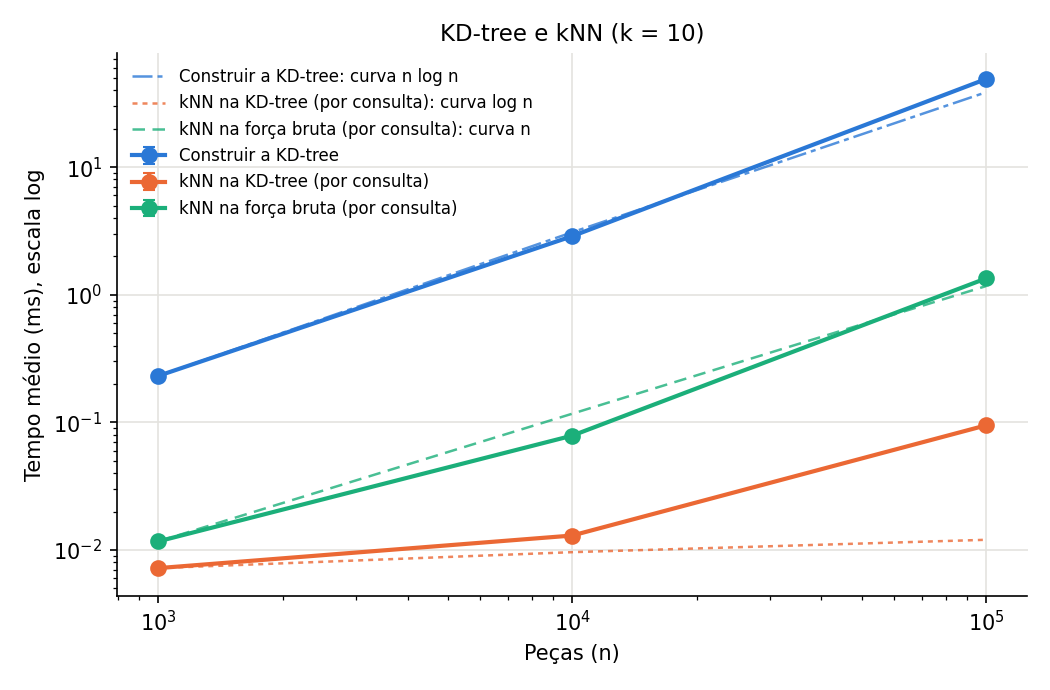
\includegraphics[width=\linewidth]{figuras/kdtree.png}\caption{KD-tree e kNN}\end{subfigure}
\begin{subfigure}{0.245\textwidth}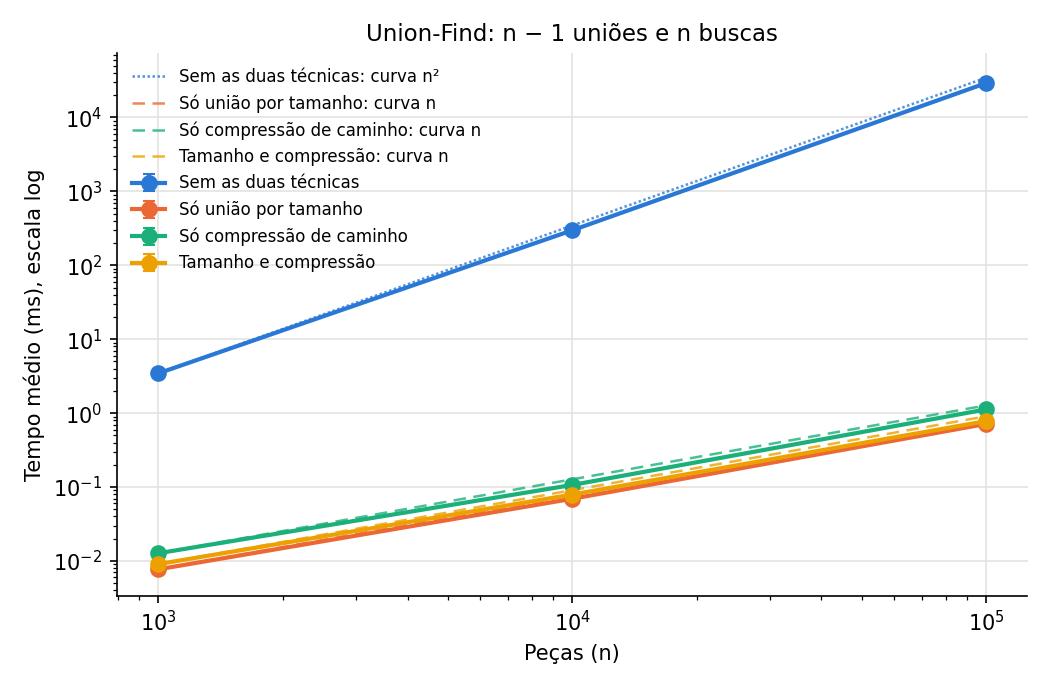
\includegraphics[width=\linewidth]{figuras/union_find.png}\caption{Union-Find}\end{subfigure}
\begin{subfigure}{0.245\textwidth}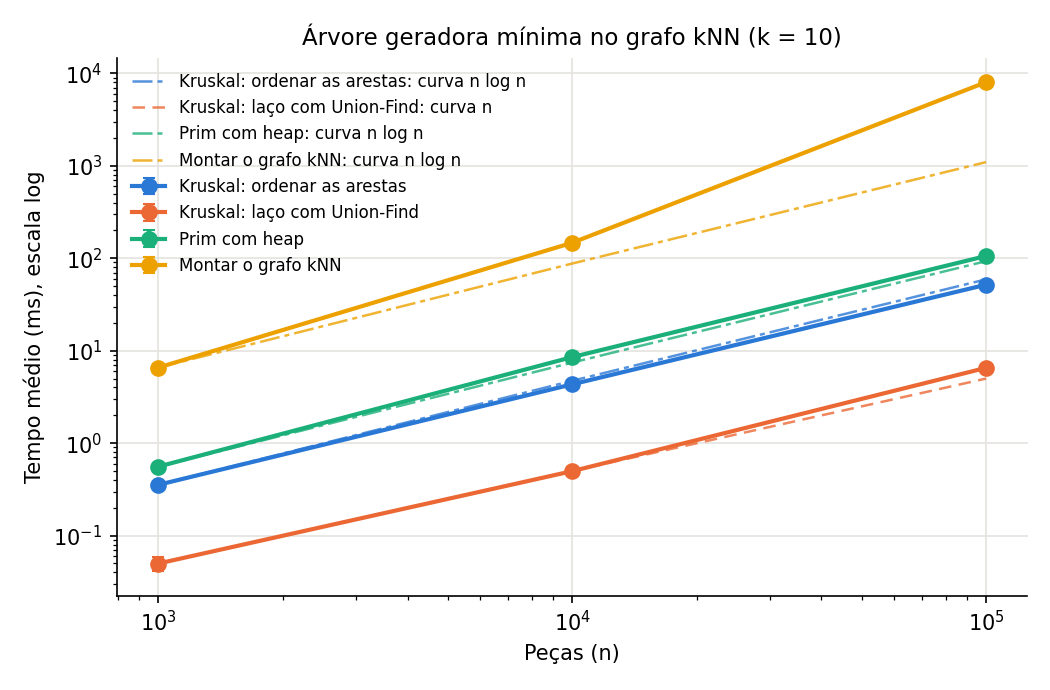
\includegraphics[width=\linewidth]{figuras/agm.png}\caption{Kruskal, Prim e grafo kNN}\end{subfigure}
\begin{subfigure}{0.245\textwidth}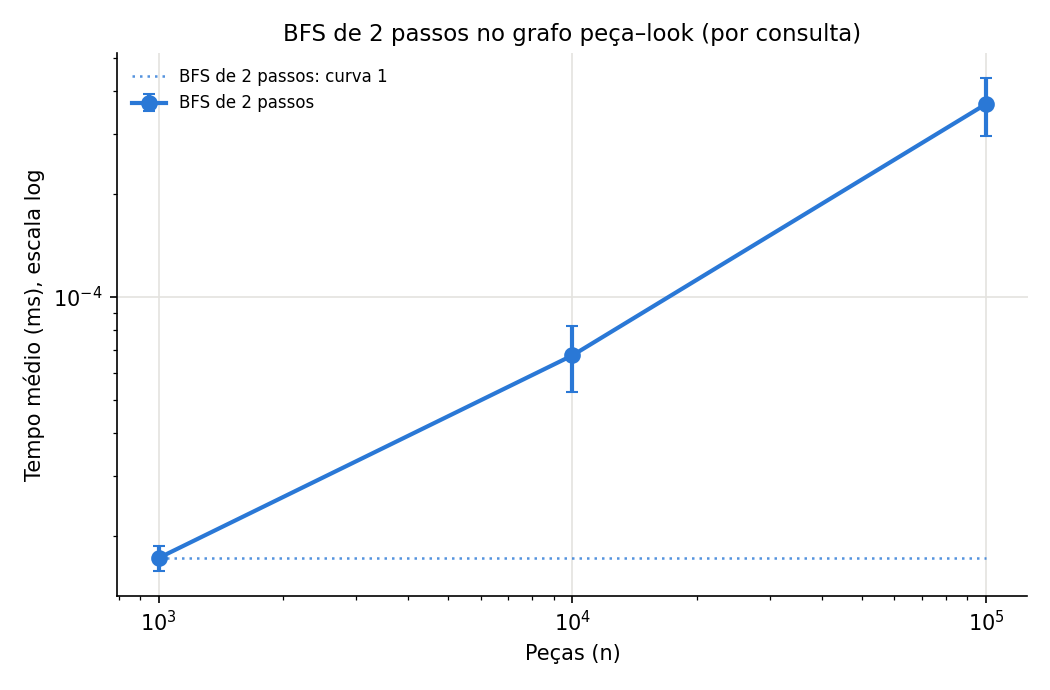
\includegraphics[width=\linewidth]{figuras/bfs.png}\caption{BFS de 2 passos}\end{subfigure}
\caption{Tempo por tamanho da base, em escala log-log, com a curva teórica tracejada.}
\label{fig:tempos}
\end{figure*}

No Union-Find sem união por tamanho e sem compressão de caminho, a sequência de teste forma uma corrente de $n$ elementos. Quando $n$ fica 10 vezes maior, o tempo fica perto de 100 vezes maior (3,458 ms, 297,6 ms e 29.204 ms), como prevê o custo quadrático. Com as duas técnicas \cite{galler1964,tarjan1975}, o crescimento é linear. Em $n = 10^5$, o tempo cai para 0,7813 ms, cerca de 37 mil vezes menos. No Kruskal, ordenar as arestas custa de 7,1 a 8,7 vezes o laço de uniões, como prevê o custo $O(E \log E)$. O Kruskal foi de 1,4 a 1,8 vez mais rápido que o Prim com heap. As duas florestas tiveram o mesmo peso.

A BFS de dois passos leva menos de 1 microssegundo por consulta. O seu custo é a soma das listas visitadas. Ele depende de em quantos looks a peça aparece e do tamanho desses looks, e não de $n$ diretamente. Na Tabela~\ref{tab:tempos}, o tempo cresce com $n$ porque os subconjuntos sorteiam peças. Com $10^3$ peças, quase todo look de treino tem só 1 peça da amostra. Com $10^5$, os looks ficam com 3 a 5 peças, e cada passo da busca visita listas maiores.

O gargalo é a montagem do grafo kNN usado pelo Kruskal. Ela faz uma busca kNN por peça e leva 8.012 ms em $n = 10^5$. Ela cresce mais que $n \log n$ pelo mesmo motivo da busca na KD-tree. Com a base maior, as etapas feitas uma vez crescem perto de $n \log n$, exceto pelo efeito dos valores repetidos. Já cada recomendação cresce de forma linear com o tamanho da categoria, pois dá nota a todas as peças dela. Uma rodada com a máquina mais carregada deu tempos de 10\% a 40\% maiores, sem mudar a forma das curvas.

\subsection{Grupos e articulações}

A Fig.~\ref{fig:grupos} mostra o grafo entre grupos, desenhado no Gephi \cite{bastian2009} com o layout ForceAtlas2 \cite{jacomy2014}. Os vértices são os 1.255 grupos de cor, estampa e formalidade dentro de cada categoria. Não usamos os grupos do Kruskal, pois neles o efeito corrente deixa 16 de 20 categorias com um grupo de mais da metade das peças. Uma aresta liga grupos de categorias diferentes com pelo menos 3 pares de peças em comum e pontos acima da mediana (0,437). O tamanho do vértice indica o número de peças. A cor destaca as articulações que separam 3 grupos ou mais. Com esse corte, 711 dos 1.255 grupos ficam com alguma aresta, todos em um único componente, ligados por 5.604 arestas. Os outros grupos ficam isolados.

\begin{figure}[t]
\centering
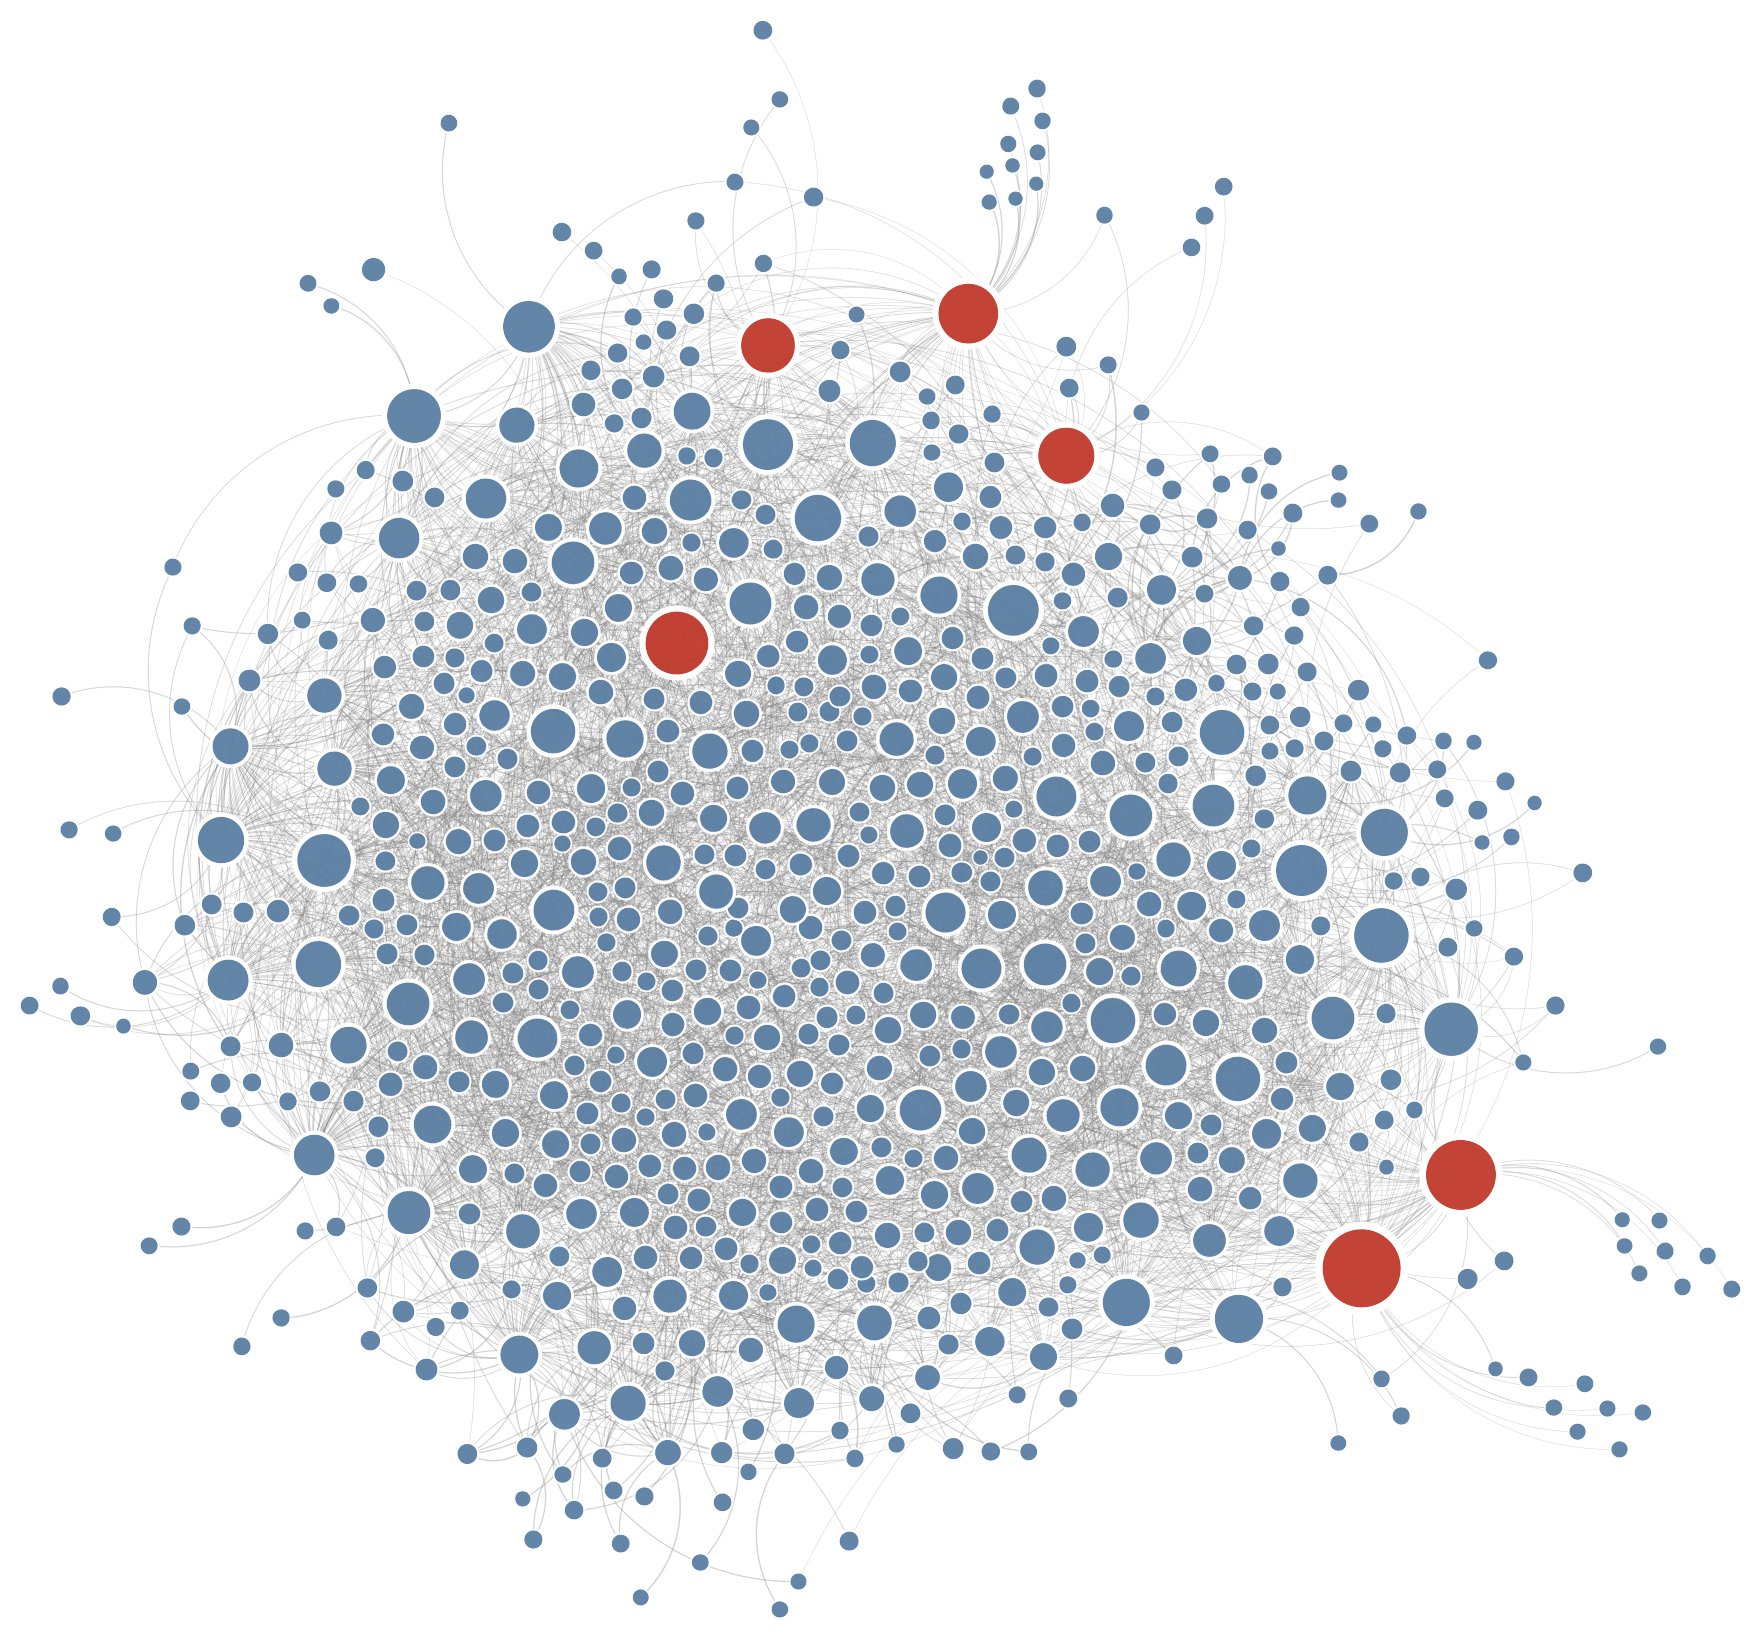
\includegraphics[width=0.72\columnwidth]{figuras/gephi.png}
\caption{Grafo entre grupos com as articulações em destaque.}
\label{fig:grupos}
\end{figure}

O algoritmo de Tarjan \cite{tarjan1972,hopcroft1973} encontrou 53 articulações e 96 pontes em 126~$\mu$s. Só 6 articulações separam 3 grupos ou mais. O resultado quase não muda com o corte. Com o primeiro quartil dos pontos (0,223), são 714 grupos ligados, 51 articulações e 6 que separam 3 ou mais. Com o terceiro quartil (0,705), são 684 grupos, 66 articulações e 7 que separam 3 ou mais. A principal é o grupo de tops brancos lisos de formalidade baixa, que separa 10 grupos. Em seguida vêm os grupos de sapatos pretos lisos e de bolsas pretas lisas de formalidade alta, com 8 cada. Peças básicas e neutras são a única ligação de alguns grupos com o resto do grafo. Esse resultado combina com a ideia de complementaridade. Uma peça básica combina com estilos diferentes e, por isso, liga grupos que não se ligariam de outra forma.

Porém, em todas as articulações, a maior parte que se separa tem um único grupo. Nenhuma ponte separa mais de 1 grupo. Assim, as articulações prendem grupos isolados na borda do grafo, e não estilos inteiros. O grau também não mostra a importância de uma articulação. O grupo de maior grau, com 96 vizinhos, separa só 2 grupos.

\subsection{Experimento registrado com a peça nova}

Depois de fixar a F, testamos 596 configurações voltadas à peça nova. A escolha usou só a validação, dividida em duas metades. A metade A escolhe e a metade B confirma. As tentativas seguiram três ideias. A primeira troca os grupos por grupos mais gerais quando há poucos pares no treino. A segunda multiplica os atributos e os grupos por $a/(1 + \text{grau})$, o que dá mais peso a essas pistas quando a peça tem pouco histórico. A terceira é uma regressão logística escrita em C++, sem biblioteca externa, que combina 13 colunas e inclui uma coluna que marca a peça nova.

Pelo Hit@10, nenhuma configuração ganhou da F nas duas metades. A melhor na metade A, com o peso por grau, chegou a 1,630\%, contra 1,123\% da F. Na metade B, ela caiu para 0,995\%, contra 1,312\% da F. A regressão logística teve o mesmo destino. Ela chegou a 1,552\% na metade A, mas na metade B a diferença para a F foi de $-0{,}026$ ponto, e pode ser sorte.

Depois, acrescentamos o FITB como critério. Essa decisão veio depois dos primeiros números e, por isso, é relatada à parte. A melhor variação por esse critério foi ao teste uma única vez, com o nome F2. Ela chegou a 41,64\% no FITB, uma diferença real de 9,60 pontos sobre a F (8,48 a 10,70), e a 37,15\% na peça nova. No Hit@10, a diferença para a F pode ser sorte, e na peça nova o valor continua em 0,000\%. A F2 fica fora das tabelas, pois o critério principal era o Hit@10.

O resultado reforça a leitura da subseção anterior. Os atributos e os grupos ajudam a escolher entre poucas opções, como no FITB. Mas eles não colocam a peça nova à frente das conhecidas na categoria inteira, porque a coocorrência e a popularidade das peças conhecidas pesam mais do que qualquer pista de semelhança.

\subsection{Ameaças à validade}

Alguns fatores limitam o alcance dos resultados. Primeiro, a base vem da Polyvore, onde os looks eram montados por usuários de um site. Esses looks refletem o gosto de quem usava o site e podem não representar o uso real das roupas. Segundo, a junção de registros repetidos usa a categoria, as cores e a legenda, e não um código de produto. Peças iguais com legendas diferentes contam como peças distintas, o que pode aumentar a fração de peças novas no teste. Terceiro, os atributos vêm de listas de palavras e do CLIP sem treino, e só a estampa passou de 70\% de acerto na conferência pela imagem. A própria base tem erros. Das 400 peças conferidas, 11 tinham a categoria errada, como um top que era um tênis. Quarto, a F foi escolhida em uma grade de 623 combinações na validação. A divisão em duas metades e o teste único reduzem, mas não eliminam, o risco de favorecer a versão escolhida.

\section{Conclusão e Próximas Etapas}
\label{sec:conc}
Este trabalho investigou até onde estruturas de dados clássicas resolvem a tarefa de completar um look. A KD-tree encontrou peças próximas sem comparar a consulta com todo o catálogo. O grafo bipartido de peças e looks, percorrido por uma BFS de dois passos, capturou a coocorrência dos looks de treino. O Union-Find e o Kruskal formaram os grupos, e o algoritmo de Tarjan apontou as articulações entre eles. Cada nota pode ser explicada pelo caminho que a produziu.

As três perguntas de pesquisa têm as respostas a seguir.

\textbf{P1. Até onde estruturas clássicas acertam a peça que falta?} A versão F alcançou Hit@10 de 1,056\% e FITB de 32,04\%, com vantagem real sobre a versão C nas duas métricas. O Hit@10 é cerca de 5,8 vezes o aleatório. Para peças que já apareceram em looks de treino, ele chega a 3,856\%, cerca de 23 vezes o aleatório.

\textbf{P2. De onde vem o acerto?} A semelhança entre peças ajuda a escolher entre poucas opções, mas não basta para ordenar milhares de candidatas. A coocorrência é a pista mais forte quando há histórico. A popularidade explica boa parte do acerto da versão final, e os grupos não trouxeram ganho que se possa medir.

\textbf{P3. O que acontece com a peça nova?} O Hit@10 da versão F cai para 0\%. A peça nova não tem arestas no grafo, então a BFS não chega até ela, e a sua popularidade vale zero. Nesse cenário, só as notas baseadas em atributos ainda superam o aleatório.

A principal descoberta do trabalho é, portanto, o viés de popularidade estrutural. Em métodos que aprendem a imitar outros modelos, o viés vem do aprendizado. Aqui, ele vem da falta de ligações no grafo. O mesmo mecanismo que ajuda a recomendar as peças conhecidas torna as peças novas invisíveis.

Além da peça nova, o trabalho tem outras limitações. Os atributos extraídos do texto e do CLIP ainda são fracos, o agrupamento pelo Kruskal sofre o efeito corrente, e a vantagem da F sobre a popularidade no Hit@10 pode ser sorte.

Cada limitação aponta uma próxima etapa. Para a peça nova, uma opção é usar direto os vetores de imagem do CLIP na KD-tree, em vez de transformar a imagem em rótulos, já que métodos visuais quase não perdem desempenho em peças sem histórico \cite{liu2020}. Outra é deixar a peça nova aproveitar a informação das peças conhecidas mais próximas na KD-tree, sem herdar junto a popularidade delas \cite{meehan2025}. Para o viés, a normalização do NGCF \cite{wang2019}, pela raiz do produto dos graus, pode ser testada no lugar da divisão simples, que piorou os resultados. Também vale medir a diversidade das listas, e não só a posição da peça certa. Para as peças repetidas, um código de produto confiável melhoraria a junção. Para os grupos, um critério que evite o efeito corrente pode produzir divisões mais úteis \cite{zahn1971}. Por fim, a análise de articulações pode ser repetida em uma base com mais looks por peça.

% Generated by IEEEtran.bst, version: 1.14 (2015/08/26)
\begin{thebibliography}{10}
\providecommand{\url}[1]{#1}
\csname url@samestyle\endcsname
\providecommand{\newblock}{\relax}
\providecommand{\bibinfo}[2]{#2}
\providecommand{\BIBentrySTDinterwordspacing}{\spaceskip=0pt\relax}
\providecommand{\BIBentryALTinterwordstretchfactor}{4}
\providecommand{\BIBentryALTinterwordspacing}{\spaceskip=\fontdimen2\font plus
\BIBentryALTinterwordstretchfactor\fontdimen3\font minus
  \fontdimen4\font\relax}
\providecommand{\BIBforeignlanguage}[2]{{%
\expandafter\ifx\csname l@#1\endcsname\relax
\typeout{** WARNING: IEEEtran.bst: No hyphenation pattern has been}%
\typeout{** loaded for the language `#1'. Using the pattern for}%
\typeout{** the default language instead.}%
\else
\language=\csname l@#1\endcsname
\fi
#2}}
\providecommand{\BIBdecl}{\relax}
\BIBdecl

\bibitem{deshpande2004}
\BIBentryALTinterwordspacing
M.~Deshpande and G.~Karypis, ``Item-based top-{N} recommendation algorithms,''
  \emph{ACM Transactions on Information Systems}, vol.~22, no.~1, p. 143–177,
  2004. [Online]. Available: \url{http://dx.doi.org/10.1145/963770.963776}
\BIBentrySTDinterwordspacing

\bibitem{han2017}
\BIBentryALTinterwordspacing
X.~Han, Z.~Wu, Y.-G. Jiang, and L.~S. Davis, ``Learning fashion compatibility
  with bidirectional lstms,'' in \emph{Proceedings of the 25th ACM
  international conference on Multimedia}, ser. MM ’17.\hskip 1em plus 0.5em
  minus 0.4em\relax ACM, 2017, p. 1078–1086. [Online]. Available:
  \url{http://dx.doi.org/10.1145/3123266.3123394}
\BIBentrySTDinterwordspacing

\bibitem{vasileva2018}
\BIBentryALTinterwordspacing
M.~I. Vasileva, B.~A. Plummer, K.~Dusad, S.~Rajpal, R.~Kumar, and D.~Forsyth,
  \emph{Learning Type-Aware Embeddings for Fashion Compatibility}.\hskip 1em
  plus 0.5em minus 0.4em\relax Springer International Publishing, 2018, p.
  405–421. [Online]. Available:
  \url{http://dx.doi.org/10.1007/978-3-030-01270-0_24}
\BIBentrySTDinterwordspacing

\bibitem{mcauley2015}
\BIBentryALTinterwordspacing
J.~McAuley, C.~Targett, Q.~Shi, and A.~van~den Hengel, ``Image-based
  recommendations on styles and substitutes,'' in \emph{Proceedings of the 38th
  International ACM SIGIR Conference on Research and Development in Information
  Retrieval}, ser. SIGIR ’15.\hskip 1em plus 0.5em minus 0.4em\relax ACM,
  2015, p. 43–52. [Online]. Available:
  \url{http://dx.doi.org/10.1145/2766462.2767755}
\BIBentrySTDinterwordspacing

\bibitem{dacrema2019}
M.~Ferrari~Dacrema, P.~Cremonesi, and D.~Jannach, ``Are we really making much
  progress? {A} worrying analysis of recent neural recommendation approaches,''
  in \emph{Proceedings of the 13th ACM Conference on Recommender Systems
  (RecSys '19)}.\hskip 1em plus 0.5em minus 0.4em\relax ACM, 2019.

\bibitem{fashionverse}
\BIBentryALTinterwordspacing
J.~Joshi, ``Fashionverse-mme (multimodal metadata enrichment),'' 2026.
  [Online]. Available: \url{https://data.mendeley.com/datasets/6sx3pbsfvz/1}
\BIBentrySTDinterwordspacing

\bibitem{efron1979}
\BIBentryALTinterwordspacing
B.~Efron, ``Bootstrap methods: Another look at the jackknife,'' \emph{The
  Annals of Statistics}, vol.~7, no.~1, p. 1–26, 1979. [Online]. Available:
  \url{http://dx.doi.org/10.1214/aos/1176344552}
\BIBentrySTDinterwordspacing

\bibitem{zenodo}
\BIBentryALTinterwordspacing
M.~E.~A. Barbosa and I.~M. Lopes, ``Atributos, grupos e divisão de looks para
  a {FashionVerse-MME},'' Zenodo, 2026. [Online]. Available:
  \url{https://doi.org/10.5281/zenodo.24372507}
\BIBentrySTDinterwordspacing

\bibitem{repositorio}
------, ``Recomendador de roupas com árvores e grafos: código-fonte,''
  \url{https://github.com/mariaeduarda-ab/recomendador--roupas-arvores-grafos},
  2026, versão v-final-2.

\bibitem{liu2020}
X.~Liu, Y.~Sun, Z.~Liu, and D.~Lin, ``Learning diverse fashion collocation by
  neural graph filtering,'' arXiv:2003.04888, 2020.

\bibitem{wang2019}
X.~Wang, X.~He, M.~Wang, F.~Feng, and T.-S. Chua, ``Neural graph collaborative
  filtering,'' in \emph{Proceedings of the 42nd International ACM SIGIR
  Conference on Research and Development in Information Retrieval}.\hskip 1em
  plus 0.5em minus 0.4em\relax ACM, 2019.

\bibitem{meehan2025}
G.~Meehan and J.~Pauwels, ``On inherited popularity bias in cold-start item
  recommendation,'' in \emph{Proceedings of the 19th ACM Conference on
  Recommender Systems (RecSys '25)}.\hskip 1em plus 0.5em minus 0.4em\relax
  ACM, 2025.

\bibitem{bentley1975}
\BIBentryALTinterwordspacing
J.~L. Bentley, ``Multidimensional binary search trees used for associative
  searching,'' \emph{Communications of the ACM}, vol.~18, no.~9, p. 509–517,
  1975. [Online]. Available: \url{http://dx.doi.org/10.1145/361002.361007}
\BIBentrySTDinterwordspacing

\bibitem{friedman1977}
\BIBentryALTinterwordspacing
J.~H. Friedman, J.~L. Bentley, and R.~A. Finkel, ``An algorithm for finding
  best matches in logarithmic expected time,'' \emph{ACM Transactions on
  Mathematical Software}, vol.~3, no.~3, p. 209–226, 1977. [Online].
  Available: \url{http://dx.doi.org/10.1145/355744.355745}
\BIBentrySTDinterwordspacing

\bibitem{galler1964}
\BIBentryALTinterwordspacing
B.~A. Galler and M.~J. Fisher, ``An improved equivalence algorithm,''
  \emph{Communications of the ACM}, vol.~7, no.~5, p. 301–303, 1964.
  [Online]. Available: \url{http://dx.doi.org/10.1145/364099.364331}
\BIBentrySTDinterwordspacing

\bibitem{tarjan1975}
\BIBentryALTinterwordspacing
R.~E. Tarjan, ``Efficiency of a good but not linear set union algorithm,''
  \emph{Journal of the ACM}, vol.~22, no.~2, p. 215–225, 1975. [Online].
  Available: \url{http://dx.doi.org/10.1145/321879.321884}
\BIBentrySTDinterwordspacing

\bibitem{kruskal1956}
\BIBentryALTinterwordspacing
J.~B. Kruskal, ``On the shortest spanning subtree of a graph and the traveling
  salesman problem,'' \emph{Proceedings of the American Mathematical Society},
  vol.~7, no.~1, p. 48–50, 1956. [Online]. Available:
  \url{http://dx.doi.org/10.1090/S0002-9939-1956-0078686-7}
\BIBentrySTDinterwordspacing

\bibitem{prim1957}
\BIBentryALTinterwordspacing
R.~C. Prim, ``Shortest connection networks and some generalizations,''
  \emph{Bell System Technical Journal}, vol.~36, no.~6, p. 1389–1401, 1957.
  [Online]. Available:
  \url{http://dx.doi.org/10.1002/j.1538-7305.1957.tb01515.x}
\BIBentrySTDinterwordspacing

\bibitem{gower1969}
\BIBentryALTinterwordspacing
J.~C. Gower and G.~J.~S. Ross, ``Minimum spanning trees and single linkage
  cluster analysis,'' \emph{Applied Statistics}, vol.~18, no.~1, p. 54–64,
  1969. [Online]. Available: \url{http://dx.doi.org/10.2307/2346439}
\BIBentrySTDinterwordspacing

\bibitem{zahn1971}
\BIBentryALTinterwordspacing
C.~Zahn, ``Graph-theoretical methods for detecting and describing gestalt
  clusters,'' \emph{IEEE Transactions on Computers}, vol. C-20, no.~1, p.
  68–86, 1971. [Online]. Available:
  \url{http://dx.doi.org/10.1109/T-C.1971.223083}
\BIBentrySTDinterwordspacing

\bibitem{tarjan1972}
\BIBentryALTinterwordspacing
R.~Tarjan, ``Depth-first search and linear graph algorithms,'' \emph{SIAM
  Journal on Computing}, vol.~1, no.~2, p. 146–160, 1972. [Online].
  Available: \url{http://dx.doi.org/10.1137/0201010}
\BIBentrySTDinterwordspacing

\bibitem{hopcroft1973}
\BIBentryALTinterwordspacing
J.~Hopcroft and R.~Tarjan, ``Algorithm 447: efficient algorithms for graph
  manipulation,'' \emph{Communications of the ACM}, vol.~16, no.~6, p.
  372–378, 1973. [Online]. Available:
  \url{http://dx.doi.org/10.1145/362248.362272}
\BIBentrySTDinterwordspacing

\bibitem{karp1972}
\BIBentryALTinterwordspacing
R.~M. Karp, \emph{Reducibility among Combinatorial Problems}.\hskip 1em plus
  0.5em minus 0.4em\relax Springer US, 1972, p. 85–103. [Online]. Available:
  \url{http://dx.doi.org/10.1007/978-1-4684-2001-2_9}
\BIBentrySTDinterwordspacing

\bibitem{bastian2009}
\BIBentryALTinterwordspacing
M.~Bastian, S.~Heymann, and M.~Jacomy, ``Gephi: An open source software for
  exploring and manipulating networks,'' \emph{Proceedings of the International
  AAAI Conference on Web and Social Media}, vol.~3, no.~1, p. 361–362, 2009.
  [Online]. Available: \url{http://dx.doi.org/10.1609/icwsm.v3i1.13937}
\BIBentrySTDinterwordspacing

\bibitem{jacomy2014}
\BIBentryALTinterwordspacing
M.~Jacomy, T.~Venturini, S.~Heymann, and M.~Bastian, ``Forceatlas2, a
  continuous graph layout algorithm for handy network visualization designed
  for the gephi software,'' \emph{PLoS ONE}, vol.~9, no.~6, p. e98679, 2014.
  [Online]. Available: \url{http://dx.doi.org/10.1371/journal.pone.0098679}
\BIBentrySTDinterwordspacing

\end{thebibliography}

\end{document}
